\documentclass[border=10pt]{standalone}

\usepackage{tikz}
\usepackage{tikzsymbols}
\usetikzlibrary{calc,patterns,shapes.geometric}

\def\centerarc[#1](#2)(#3:#4:#5){\draw[#1] ($(#2)+({#5*cos(#3)},{#5*sin(#3)})$) arc (#3:#4:#5);}

\begin{document}
	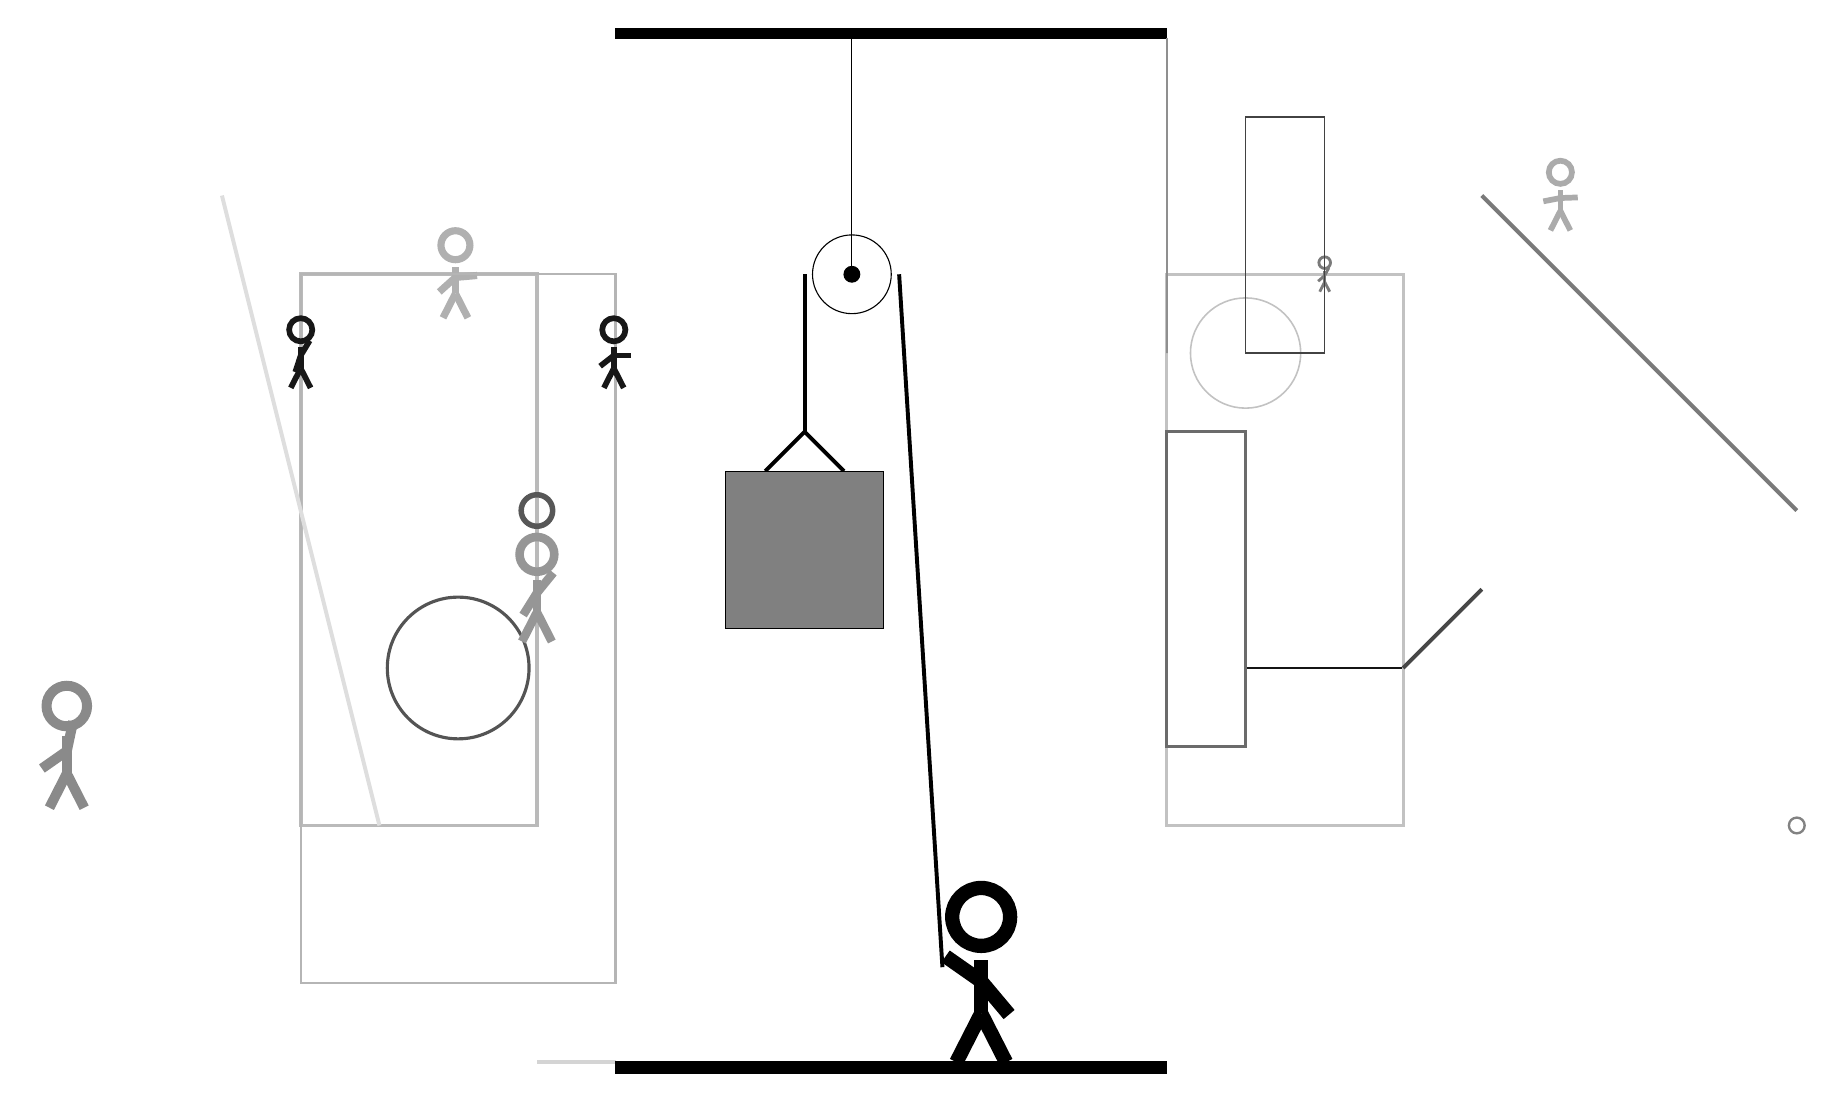
\begin{tikzpicture}
		%%%%% START %%%%%
		
		\draw[fill=black] (-2, 10) rectangle (5, 10.125);
		
		\draw (1, 7) circle (0.5);
		\draw[fill=black] (1, 7) circle (0.1);
		\draw (1, 10) -- (1, 7);
		
		\draw[line width=0.5mm] (-0.1, 4.5) -- (0.4, 5.0) -- (0.9, 4.5);
		\draw[fill=black!50] (-0.6, 4.5) rectangle (1.4, 2.5);
		
		\draw[line width=0.5mm] (0.4, 7) -- (0.4, 5.0);
		\centerarc[line width=0.5mm](1, 7)(0:180:0.6);
		\draw[line width=0.5mm](1.6, 7) -- (2.15, -1.8);
		
		\draw [line width=0.2mm, color=black!24](6, 6) circle (0.7);
		
		\draw[line width=0.3mm, color=black!92] (6, 2) rectangle (8, 2);
		\draw[line width=0.4mm, color=black!24] (5, 0) rectangle (8, 7);
		\draw[line width=0.5mm, color=black!27] (-3, 7) rectangle (-6, 0);
		\node[line width=0.4mm, color=black!33] at (10, 8) {\Strichmaxerl[4][11][2]};
		
		\draw[line width=0.2mm, color=black!44] (5, 6) rectangle (5, 10);
		\node[line width=0.6mm, color=black!31] at (-4, 7) {\Strichmaxerl[5][42][5]};
		
		\draw [line width=0.3mm, color=black!49](13, 0) circle (0.1);
		\draw [line width=0.4mm, color=black!67](-4, 2) circle (0.9);
		\draw[line width=0.3mm, color=black!29] (-2, 7) rectangle (-6, -2);
		
		\draw[line width=0.5mm, color=black!13](-7, 8) -- (-5, 0);
		\draw[line width=0.5mm, color=black!72](8, 2) -- (9, 3);
		\node[line width=0.2mm, color=black!52] at (7, 7) {\Strichmaxerl[2][41][62]};
		
		\node[line width=0.5mm, color=black!91] at (-2, 6) {\Strichmaxerl[4][38][0]};
		\draw[line width=0.5mm, color=black!17](-2, -3) -- (-3, -3);
		\node[line width=0.2mm, color=black!91] at (-6, 6) {\Strichmaxerl[4][72][59]};
		
		\node[line width=0.4mm, color=black!46] at (-9, 1) {\Strichmaxerl[7][35][78]};
		
		\draw [line width=0.7mm, color=black!66](-3, 4) circle (0.2);
		\node[line width=0.3mm, color=black!41] at (-3, 3) {\Strichmaxerl[6][58][51]};
		\draw[line width=0.2mm, color=black!74] (7, 6) rectangle (6, 9);
		\draw[line width=0.4mm, color=black!58] (6, 1) rectangle (5, 5);
		
		\draw[line width=0.5mm, color=black!52](9, 8) -- (13, 4);
		
		\node at (2.6, -1.9) {\Strichmaxerl[10][-35][-50]};
		
		\draw[fill=black] (-2, -3) rectangle (5, -3.15);
		
		%%%%% END %%%%%
	\end{tikzpicture}
\end{document}